\chapter{ArUco localization}\label{ch:aruco}
\sloppy

The Tello has no GPS, no motion capture and no usable optical flow over the plain floor of the bedroom. Its only
\emph{absolute} position sensor is its forward camera looking at 44 printed ArUco markers glued on the walls. This
chapter follows one camera image from the moment it arrives on \topic{/tello/image\_raw} until it becomes a pose of
the drone body on \topic{/aruco/pose}, and explains every function of the package
\file{src/aruco\_localization/} on the way, with the mathematics behind it and the numbers actually used.

\begin{intuition}
The marker map (\file{config/markers.yaml}) tells us where, in the room, every corner of every marker is: a list of
known 3D points. The camera image tells us where those same corners appear in pixels: a list of 2D points. Knowing
how the lens maps 3D to 2D (the calibration, \file{config/tello\_camera.yaml}), there is only one camera position and
orientation that makes the known 3D corners land on the observed pixels. Finding it is the
\emph{Perspective-n-Point} (PnP) problem. The drone body is then 5~cm behind the camera, rotated by a fixed mount.
Everything else in this chapter is about doing that fast, and about refusing the answer when it is wrong.
\end{intuition}

\section{The package at a glance}

\begin{table}[h]
\centering\small
\begin{tabular}{@{}lll@{}}
\toprule
File & Lines & Role \\
\midrule
\file{aruco\_localizer.py} & 353 & Node \code{aruco\_localizer}: detection, joint PnP, checks, publishing \\
\file{marker\_map.py} & 108 & No ROS: load the YAML map, marker corners, rotation helpers \\
\file{marker\_map\_publisher.py} & 205 & Node \code{marker\_map\_publisher}: static TFs and RViz decorations \\
\file{setup.py}, \file{package.xml} & & \code{ament\_python} package, two console scripts \\
\bottomrule
\end{tabular}
\end{table}

\file{setup.py} declares the Python package \code{aruco\_localization} and two \code{console\_scripts} entry points:
\begin{lstlisting}
marker_map_publisher = aruco_localization.marker_map_publisher:main
aruco_localizer = aruco_localization.aruco_localizer:main
\end{lstlisting}
these are the \code{executable} names used by
\file{src/tello\_driver/launch/real.launch.py}. It installs only \file{package.xml} and the ament resource marker; the
configuration files are not installed but passed as absolute paths by the launch file (parameter
\code{markers\_file}). \file{package.xml} (format~3, build type \code{ament\_python}) lists only run-time
dependencies: \code{rclpy}, \code{sensor\_msgs}, \code{geometry\_msgs}, \code{nav\_msgs}, \code{visualization\_msgs},
\code{std\_msgs}, \code{tf2\_ros}, \code{cv\_bridge}, \code{python3-opencv}, \code{python3-yaml}. The code is written to
work with both the Ubuntu 24.04 system OpenCV (4.6, old ArUco API) and OpenCV $\geq$ 4.7 (new \code{ArucoDetector}
class).

The launch file starts the two nodes with these parameters (\file{real.launch.py}, lines 51--58):
\begin{itemize}
\item \code{marker\_map\_publisher}: \code{markers\_file}, \code{room\_mesh} (the phone scan, if found),
  \code{flight\_zone\_file} (by default \file{config/flight\_zone\_band.yaml});
\item \code{aruco\_localizer}: \code{markers\_file}, \code{child\_frame = "base\_link\_aruco"},
  \code{debug\_every\_n = 3}, \code{debug\_scale = 0.5}.
\end{itemize}

\subsection{Topics and frames}

\begin{table}[h]
\centering\footnotesize
\begin{tabularx}{\textwidth}{@{}>{\raggedright\arraybackslash}p{5.4cm}>{\raggedright\arraybackslash}p{3.5cm}>{\raggedright\arraybackslash}p{2.7cm}X@{}}
\toprule
Topic / frame & Type & Publisher (depth) & Consumers \\
\midrule
\topic{/tello/image\_raw} & \code{Image} rgb8 & driver (5) & localizer (depth 1) \\
\topic{/tello/camera\_info} & \code{CameraInfo} & driver (5) & localizer (5) \\
\topic{/aruco/pose} & \code{PoseWithCov.Stamped} & localizer (10) & EKF, missions, recorder \\
\topic{/aruco/nearest\_marker} & \code{Float32} (m) & localizer (5) & driver wall guard \\
\topic{/aruco/ids} & \code{String} & localizer (5) & \code{patrol.py} \\
\topic{/aruco/debug\_image} & \code{Image} bgr8 & localizer (2) & RViz, \code{session\_recorder} \\
\topic{/aruco/path} & \code{nav\_msgs/Path} & localizer (2) & (not shown in \file{real.rviz}) \\
\topic{/aruco/sight\_lines} & \code{Marker} & localizer (5) & RViz \\
TF \topic{map}$\to$\topic{base\_link\_aruco} & & localizer & RViz \\
TF \topic{map}$\to$\topic{aruco\_<id>} (static) & & map publisher & RViz, anyone \\
TF \topic{base\_link}$\to$ \topic{tello\_camera\_optical} (static) & & map publisher & localizer, RViz \\
\topic{/aruco/map\_markers} & \code{MarkerArray} & map publisher (latched) & RViz \\
\topic{/tello/body\_markers} & \code{MarkerArray} & map pub. (latched, 1 Hz) & RViz \\
\topic{/room/mesh} & \code{Marker} & map publisher (latched) & RViz \\
\topic{/room/flight\_zone} & \code{MarkerArray} & map pub. (latched, 0.5 Hz) & RViz \\
\topic{/room/free\_space} & \code{OccupancyGrid} & map publisher (latched) & RViz \\
\bottomrule
\end{tabularx}
\end{table}

``Latched'' means a QoS profile with \code{depth=1} and \code{DurabilityPolicy.TRANSIENT\_LOCAL}: a subscriber that
starts later (RViz opened after the launch) still receives the last message. The consumers were checked in the code:
\file{core/ekf\_node.py}:53 subscribes \topic{/aruco/pose} with depth 20; \file{core/driver.py}:130 forwards
\topic{/aruco/nearest\_marker} to \code{safety.on\_nearest\_marker}; \file{missions/patrol.py}:61 parses \topic{/aruco/ids};
\file{core/session\_recorder.py}:42--43 saves the debug image (at most one per second) and the poses;
\file{missions/tour.py}:77 and \file{missions/base.py} also read \topic{/aruco/pose}.

\section{The configuration files}

\subsection{\texttt{config/markers.yaml}: the marker map}

This file is the single source of truth for the marker layout, used by the real localizer, the fake camera of the
simulator (\file{sim/fake\_world.py}) and the map publisher. It was produced by \file{tools/room\_mapper.py}: 244 hand-held
photos, then a bundle adjustment (reprojection RMS 1.13~px) that solved all marker poses at once. Its format:

\begin{lstlisting}
dictionary: DICT_6X6_50
marker_size: 0.1889     # side of the black square (m); per-marker 'size' overrides it
room: {size_x: 4.01, size_y: 4.89, height: 3.42}   # simulator only
markers:
  - {id: 49, x: 0.000, y: 0.000, z: 1.950, yaw_deg: 90.0,
     q: [-0.0009, 0.7095, 0.7047, 0.0009]}   # views 130, tilt 0.4 deg
  ...
\end{lstlisting}

\begin{itemize}
\item \code{dictionary}: the OpenCV predefined dictionary name, \code{DICT\_6X6\_50}: $6\times 6$ data bits inside a
  one-cell black border, 50 ids (0--49), chosen far apart in Hamming distance so that a few misread bits are still
  identified, and so that no code equals another one rotated by $90^\circ$; the detection therefore also gives the
  marker's in-plane orientation (which corner is top-left).
\item \code{marker\_size}: $\ell = 0.1889$~m. The markers were meant to be 20~cm but the printer shrank them by about
  6\,\%. Every metric distance in the system scales with this number (PnP recovers the scene up to the scale given by
  the object points).
\item One entry per marker: centre $(x,y,z)$ in \topic{map} (metres), \code{yaw\_deg} (direction the marker faces,
  used only if \code{q} is absent) and \code{q} $= (q_x,q_y,q_z,q_w)$, the full measured orientation of the marker
  frame in \topic{map}. Optional \code{size}.
\end{itemize}

The file contains 44 markers. The \topic{map} frame has its origin on the floor below marker 49, $y$ pointing out of
marker 49's wall into the room, $z$ up. Two entries carry history worth knowing: marker 39 fell on Nov~13 and was
re-located from 4 flight frames; marker 18 was ``added Nov 16 by hand, NOT measured'' (same orientation as 46). The
\code{room} block is only used by the simulator.

Marker frame convention (OpenCV): origin at the centre of the black square, $x$ to the right and $y$ up as seen from
the front, $z$ out of the wall towards the camera. With $\mathbf R_k$ the marker's axes expressed in \topic{map} and
$\mathbf t_k$ its centre, the four corners in detection order (top-left, top-right, bottom-right, bottom-left) are
\begin{equation}
\mathbf X_{k,j} = \mathbf t_k + \mathbf R_k \,\mathbf c_j,\qquad
\mathbf c_{1..4} = \tfrac{\ell}{2}\begin{bmatrix}-1\\1\\0\end{bmatrix},\
\tfrac{\ell}{2}\begin{bmatrix}1\\1\\0\end{bmatrix},\
\tfrac{\ell}{2}\begin{bmatrix}1\\-1\\0\end{bmatrix},\
\tfrac{\ell}{2}\begin{bmatrix}-1\\-1\\0\end{bmatrix}.
\label{eq:corners}
\end{equation}

\subsection{\texttt{config/tello\_camera.yaml}: intrinsics and distortion}

Standard ROS \code{camera\_info} YAML, produced by \file{tools/calibrate\_camera.py} with a checkerboard (26 sharp
views, RMS 0.236~px, Nov~9). The driver loads it (\code{camera\_info\_file}, \file{core/driver.py}:278) and republishes it
on \topic{/tello/camera\_info} with every frame. Values for the $960\times 720$ stream:
\begin{equation}
\mathbf K = \begin{bmatrix} f_x & 0 & c_x\\ 0 & f_y & c_y\\ 0&0&1\end{bmatrix}
=\begin{bmatrix} 910.47 & 0 & 466.65\\ 0 & 913.55 & 363.89\\ 0&0&1\end{bmatrix},
\end{equation}
\begin{equation}
\mathbf D = (k_1,k_2,p_1,p_2,k_3) = (-0.0386,\ 0.0816,\ -0.00129,\ -0.00525,\ 0).
\end{equation}
The distortion model is \code{plumb\_bob} (radial $k_1,k_2,k_3$ and tangential $p_1,p_2$; $k_3$ fixed to 0 during the
calibration). The rectification matrix is the identity and the projection matrix is $[\mathbf K\,|\,\mathbf 0]$: the
image is never rectified, OpenCV takes $\mathbf D$ into account inside \code{solvePnP} and \code{projectPoints}.
The field of view follows from $\mathbf K$: horizontally $2\arctan(480/910.5)=55.6^\circ$, vertically
$2\arctan(360/913.5)=43.0^\circ$, exactly the values used to draw the camera frustum in RViz
(\file{marker\_map\_publisher.py}:131).

\section{Background: how a calibrated camera measures a pose}

\subsection{The pinhole model with distortion}

Let $\mathbf X$ be a point in the \topic{map} frame and $({}^c\mathbf R_m, {}^c\mathbf t_m)$ the transform from
\topic{map} to the camera optical frame (this is exactly what OpenCV calls \code{rvec, tvec}). The camera frame point
is $\mathbf X_c = {}^c\mathbf R_m \mathbf X + {}^c\mathbf t_m = (X_c,Y_c,Z_c)$. The optical frame has $z$ forward
along the optical axis, $x$ to the right, $y$ down. Projection:
\begin{align}
x &= X_c/Z_c,\qquad y = Y_c/Z_c, \qquad r^2 = x^2+y^2,\\
x_d &= x\,(1+k_1r^2+k_2r^4+k_3r^6) + 2p_1xy + p_2(r^2+2x^2),\\
y_d &= y\,(1+k_1r^2+k_2r^4+k_3r^6) + p_1(r^2+2y^2) + 2p_2xy,\\
\begin{bmatrix}u\\v\\1\end{bmatrix} &= \mathbf K\begin{bmatrix}x_d\\y_d\\1\end{bmatrix}
\quad\Longleftrightarrow\quad u = f_x x_d + c_x,\ \ v = f_y y_d + c_y .
\end{align}
We write this whole chain $\pi(\mathbf X; \mathbf R,\mathbf t,\mathbf K,\mathbf D)$. With the numbers of the
Tello, a point at normalised radius $r\approx 0.45$ (about 400~px from the centre) is moved by
$f_x\, r\, |k_1r^2+k_2r^4| \approx 910\times 0.45\times 0.0045 \approx 1.8$~px by the radial terms: small, but of the
same order as the 3~px acceptance threshold used below, which is why $\mathbf D$ is passed everywhere.

\subsection{Does it use how many pixels the marker takes? Where does distance come from?}

Without distortion, a segment of length $\ell$ facing the camera at depth $Z$ appears $s = f\ell/Z$ pixels long
(similar triangles). With $f_x\ell = 910.47\times 0.1889 = 172.0$~px\,m, a marker is 172~px wide at 1~m, 86~px at 2~m,
57~px at 3~m. This is the \emph{only} place where ``how many pixels the marker takes'' is used explicitly: the
proximity sensor \topic{/aruco/nearest\_marker} computes $d = f_x\ell/s_{\max}$ (section~\ref{sec:nearest}).

The pose itself does \emph{not} use the apparent size as a separate cue; it is implicit in PnP. The object points are
in metres and $\mathbf K$ converts metres-at-unit-depth into pixels, so the only way to make four corners
separated by 0.1889~m appear $s$~px apart is to put them at depth $\approx f\ell/s$. Calibration is what makes this
metric: $f_x$ (in pixels) is the conversion factor between angles and pixels, and $\ell$ the conversion between the
map and metres. A 1\,\% error on $f_x$ or on $\ell$ gives a 1\,\% error on every distance. The sensitivity is also
clear: $\delta Z/Z = \delta s/s$, so one pixel of corner error on a marker 86~px wide (2~m) is a 1.2\,\% (2.3~cm)
depth error, while the same pixel moves the lateral position by only $Z/f_x = 2.2$~mm. PnP is much better laterally
than in depth, and it gets better the more spread-out the corners are in the image.

\subsection{Perspective-n-Point}

Given $N$ correspondences between object points $\mathbf X_i$ (3D, \topic{map} frame, from the marker map) and image
points $\mathbf p_i=(u_i,v_i)$ (detected corners, pixels), PnP finds
\begin{equation}
({}^c\mathbf R_m,{}^c\mathbf t_m) = \arg\min_{\mathbf R\in SO(3),\,\mathbf t}
\sum_{i=1}^{N}\big\lVert \mathbf p_i - \pi(\mathbf X_i;\mathbf R,\mathbf t,\mathbf K,\mathbf D)\big\rVert^2 .
\label{eq:pnp}
\end{equation}
A pose has 6 unknowns and each correspondence gives 2 equations: 3 points are the theoretical minimum (with up to 4
solutions), 4 coplanar points (one marker) already give a unique solution in exact arithmetic but, as we will see, a
near-ambiguity in practice. The code uses three OpenCV solvers:
\begin{itemize}
\item \code{SOLVEPNP\_SQPNP} (Terzakis and Lourakis, 2020): casts \eqref{eq:pnp} (in its algebraic, undistorted
  form) as a quadratically constrained problem over the 9 entries of $\mathbf R$ and finds the \emph{global} minimum by
  sequential quadratic programming from several starting points. Works for any $N\geq 3$, planar or not. Used for
  several markers. Fallback \code{SOLVEPNP\_ITERATIVE} (DLT/homography init + Levenberg--Marquardt) if the constant does
  not exist.
\item \code{SOLVEPNP\_IPPE\_SQUARE} (Collins and Bartoli, 2014): ``Infinitesimal Plane-based Pose Estimation''
  specialised for a square of known side with its four corners in the exact order of equation~\eqref{eq:corners}
  expressed in the marker's own frame. It computes the homography of the square and returns \emph{both} local minima of
  the planar pose problem, sorted, with their reprojection errors. Used for one marker, via
  \code{solvePnPGeneric}, which returns all solutions.
\item \code{solvePnPRefineLM}: Levenberg--Marquardt refinement of \eqref{eq:pnp} with the full distortion model,
  started from the solver's answer. Always applied last.
\end{itemize}

\code{rvec} is an axis-angle vector (direction = rotation axis, norm = angle in radians); \code{cv2.Rodrigues}
converts it to and from ${}^c\mathbf R_m$. \code{tvec} is ${}^c\mathbf t_m$: the \topic{map} origin expressed in the
camera frame. Neither is the camera position: that is $\mathbf c = -{}^c\mathbf R_m^\top\, {}^c\mathbf t_m$.

\subsection{The chain of transforms}

Write ${}^a\mathbf T_b$ for the $4\times 4$ homogeneous transform that maps coordinates in frame $b$ to frame $a$
(equivalently, the pose of $b$ in $a$). PnP gives ${}^c\mathbf T_m$; its inverse is the camera pose in the map:
\begin{equation}
{}^c\mathbf T_m = \begin{bmatrix} {}^c\mathbf R_m & {}^c\mathbf t_m\\ \mathbf 0^\top & 1\end{bmatrix},
\qquad
{}^m\mathbf T_c = ({}^c\mathbf T_m)^{-1} = \begin{bmatrix} {}^c\mathbf R_m^\top & -{}^c\mathbf R_m^\top\,{}^c\mathbf t_m\\
\mathbf 0^\top & 1\end{bmatrix}.
\end{equation}
The camera is fixed on the body (\topic{base\_link}: $x$ forward, $y$ left, $z$ up) by the static transform
${}^b\mathbf T_c$ published by \code{marker\_map\_publisher}:
\begin{equation}
{}^b\mathbf T_c = \begin{bmatrix} {}^b\mathbf R_c & {}^b\mathbf t_c\\ \mathbf 0^\top & 1\end{bmatrix},\qquad
{}^b\mathbf R_c = \begin{bmatrix} 0&0&1\\ -1&0&0\\ 0&-1&0\end{bmatrix},\qquad
{}^b\mathbf t_c = \begin{bmatrix}0.05\\0\\0\end{bmatrix}.
\label{eq:mount}
\end{equation}
The columns of ${}^b\mathbf R_c$ are the optical axes in body coordinates: optical $x$ (right) $=-y_b$, optical $y$
(down) $=-z_b$, optical $z$ (forward) $=x_b$. The drone body pose is then
\begin{equation}
{}^m\mathbf T_b = {}^m\mathbf T_c\,({}^b\mathbf T_c)^{-1},
\qquad\text{i.e.}\qquad
{}^m\mathbf R_b = {}^m\mathbf R_c\,{}^b\mathbf R_c^\top,\quad
{}^m\mathbf t_b = {}^m\mathbf t_c - {}^m\mathbf R_b\,{}^b\mathbf t_c .
\label{eq:body}
\end{equation}
Including the markers, the full chain the localizer implicitly closes is
${}^m\mathbf T_b = {}^m\mathbf T_{k}\;{}^{k}\mathbf T_c\;{}^c\mathbf T_b$ for every marker $k$ in view, where
${}^m\mathbf T_k$ comes from the YAML (and is the static TF \topic{map}$\to$\topic{aruco\_k}) and ${}^k\mathbf T_c$ is
what a single-marker solver would measure. The multi-marker code does not compute ${}^k\mathbf T_c$ at all: it puts
the corners directly in \topic{map} coordinates (equation~\eqref{eq:corners}) so PnP returns ${}^c\mathbf T_m$ in one
step. The single-marker code does compute ${}^k\mathbf T_c$ (IPPE needs the marker frame) and then composes with
${}^m\mathbf T_k$ (section~\ref{sec:single}).

Orientation: the roll, pitch, yaw of the drone are those of ${}^m\mathbf R_b$. The localizer publishes it as a
quaternion; the EKF extracts only the yaw, $\psi = \operatorname{atan2}(2(q_wq_z+q_xq_y),\,1-2(q_y^2+q_z^2))$
(\file{core/ekf\_node.py}:70), which equals $\operatorname{atan2}(R_{21},R_{11})$ of ${}^m\mathbf R_b$.

\section{PnP step by step, with the real camera}\label{sec:pnp-steps}

This section answers, with numbers, the questions ``what exactly is computed when the drone sees a marker'',
``why four corners and not the centre'', ``what is this mirror ambiguity'' and ``why a solver''. All numbers use the
real calibration of \file{config/tello\_camera.yaml} ($f_x = 910.47$, $f_y = 913.55$, $c_x = 466.65$,
$c_y = 363.89$~px), without distortion for clarity. They are produced by \file{docs/book/figures/pnp\_example.py}.

\begin{keypoint}
\textbf{This is not epipolar geometry.} Epipolar geometry (epipolar plane, essential matrix $E$) relates
\emph{two images} of the same unknown 3D point. Here there is \emph{one} image and points whose 3D position is
\emph{already known} (the marker corners, from \file{markers.yaml}). The problem is Perspective-n-Point: find
where the camera is so that the known 3D points fall on the measured pixels.
\end{keypoint}

\subsection{What is known, what is unknown}

\begin{center}
\begin{tabular}{@{}lll@{}}
\toprule
& What & Where it comes from \\
\midrule
known & 3D position $P_k$ of every corner, in \code{map} & \file{markers.yaml} (centre $t_m$, axes $R_m$, side $\ell$) \\
known & pixel $p_k = (u_k, v_k)$ of every corner & the detector (sub-pixel corners) \\
known & $K$, $D$ & the calibration \\
\textbf{unknown} & \textbf{one} rotation $R$ and \textbf{one} translation $t$ & what PnP solves \\
\bottomrule
\end{tabular}
\end{center}

The unknown is \emph{not} ``one transformation per point''. It is a single rigid transformation, the pose of the
camera, that is the same for all the points: a corner $P_k$ of the room is seen in the camera frame at
\begin{equation}
P_k^{c} = R\,P_k + t = \begin{bmatrix} X_k \\ Y_k \\ Z_k \end{bmatrix}
\qquad\text{(camera frame: $x$ right, $y$ down, $z$ forward)}.
\end{equation}
$R$ has 3 degrees of freedom and $t$ has 3: \textbf{6 unknown numbers in total}, whatever the number of points.
The points are the \emph{measurements} that pin these 6 numbers down.

\subsection{Perspective = dividing by the depth}

A point in front of the camera lands on the pixel
\begin{equation}
u = f_x \frac{X}{Z} + c_x, \qquad v = f_y \frac{Y}{Z} + c_y .
\label{eq:pinhole}
\end{equation}
That division by $Z$ \emph{is} perspective: the same object twice as far is half as big in the image.

\paragraph{Example 1: a marker facing the camera.} Its corners are at $X, Y = \pm\ell/2 = \pm 0.0945$~m. At
$Z = 2$~m: $u = 910.47 \times (\pm 0.0945)/2 + 466.65 = 509.6$ or $423.7$, so the marker is $86.0$~px wide. At
$Z = 1$~m it is $172.0$~px wide. The size gives the distance:
$d = f_x \ell / (\text{width in px}) = 910.47 \times 0.1889 / 86.0 = 2.00$~m. This is exactly the formula of
\topic{/aruco/nearest\_marker}.

\paragraph{Example 2: the same marker turned by $20^\circ$.} Now one vertical edge is closer to the camera than the
other ($Z$ differs by $\ell\sin 20^\circ = 6.5$~cm). The closer edge looks taller, the far one shorter, and the
marker looks narrower: the square becomes a \emph{trapezoid}.

\begin{center}
\begin{tabular}{@{}lccc@{}}
\toprule
Marker at 2 m & width (px) & left edge (px) & right edge (px) \\
\midrule
facing the camera & 86.0 & 86.3 & 86.3 \\
turned $+20^\circ$ & 80.8 & 84.9 & 87.7 \\
turned $-20^\circ$ & 80.8 & 87.7 & 84.9 \\
\bottomrule
\end{tabular}
\end{center}

The width shrinks by $\cos 20^\circ$ (it tells \emph{how much} the marker is turned), and the difference between the two
edges (here $2.8$~px) tells \emph{which way}. That is the whole ``perspective transformation'': the shape of the
quadrilateral in the image encodes the angle, its size encodes the distance, its position in the image encodes the
direction.

\begin{figure}[h]
\centering
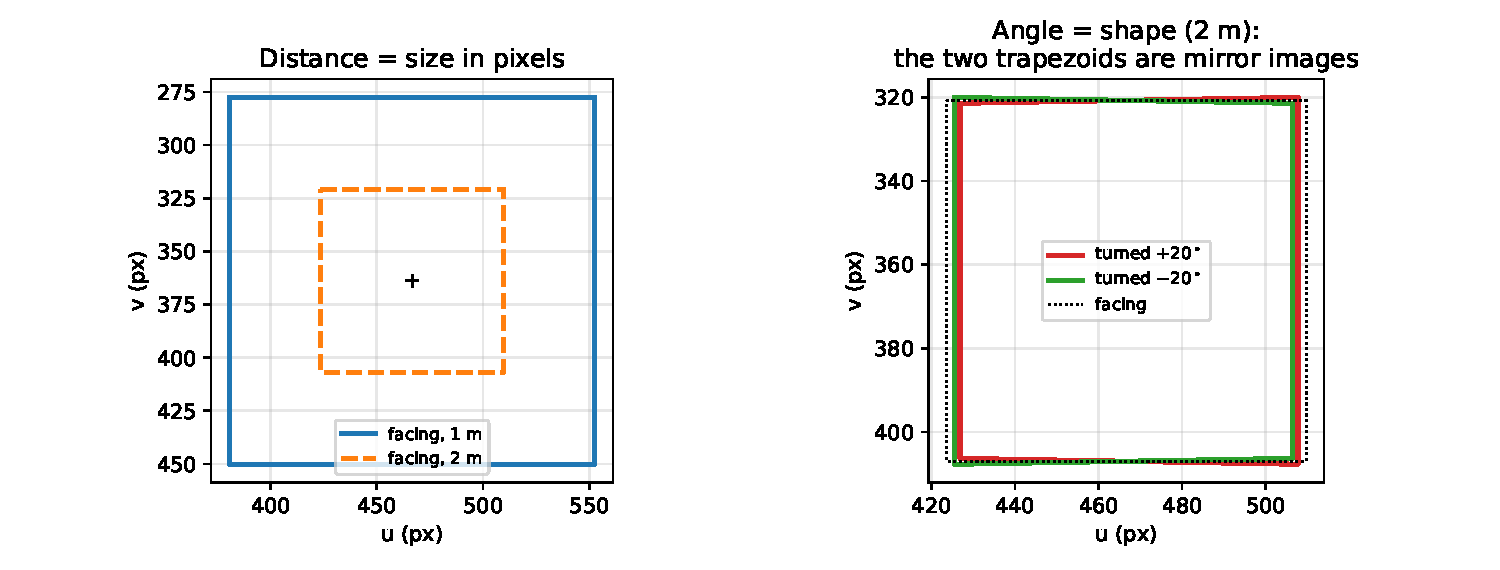
\includegraphics[width=\textwidth]{figures/pnp_perspective.pdf}
\caption{Left: distance = size (1 m vs 2 m). Right: angle = shape. Turned $+20^\circ$ and $-20^\circ$ give mirror
trapezoids that differ by only $\approx 1.4$~px per corner.}
\end{figure}

\subsection{Counting equations: why four corners and not the centre}

Each pair ``known 3D point $\leftrightarrow$ measured pixel'' gives \textbf{2 equations} (its $u$ and its $v$,
eq.~\ref{eq:pinhole}). There are \textbf{6 unknowns}.

\begin{center}
\begin{tabular}{@{}lll@{}}
\toprule
Points used & Equations & What it fixes \\
\midrule
centre of 1 marker & 2 & only a \emph{ray}: the camera is somewhere on the line through the marker centre \\
2 points & 4 & a one-parameter family of poses \\
3 points & 6 & a finite set: up to 4 poses (the classical P3P problem) \\
4 corners of 1 marker & 8 & one pose in theory, but two nearly equivalent in practice (next subsection) \\
4 corners of $n \geq 2$ markers & $8n$ & one well-determined pose \\
\bottomrule
\end{tabular}
\end{center}

With centres only, the drone would need at least three markers in view at the same time to compute anything, and
it would throw away the size and shape of each marker (the distance and angle information of the examples above).
The four corners carry all of it, so one marker is already enough.

\paragraph{Several markers: one problem.} All corners of all visible markers are expressed in the same \code{map}
frame, so they are simply stacked: 3 markers give 12 pairs and 24 equations for the same 6 unknowns. The angle
gets much better because the points are spread out: the angle error is roughly (pixel error) / (pixel distance
between the points). For a corner error of $0.5$~px at 2~m: one marker (corners $86$~px apart) gives
$0.5/86 = 0.006$~rad $= 0.33^\circ$; two markers 1~m apart ($455$~px) give $0.06^\circ$. It is like measuring a slope
with a long ruler instead of a short one.

\subsection{The mirror ambiguity of a single marker}

A 19~cm marker seen from 1--3~m is small compared with its distance. The perspective effect that tells
``turned left'' from ``turned right'' is then tiny: in the table above, turning the marker $+20^\circ$ or $-20^\circ$
changes each corner by only about $1.4$~px, and the detector's corners have $\approx 0.3$~px of noise. Two camera
poses explain the 4 corners almost equally well. In the map they are symmetric about the line of sight: the camera
is either to the left or to the right of the marker's normal.

\paragraph{Example 3: what OpenCV returns.} Marker $0.5$~m to the right of the optical axis, 2~m away, turned
$20^\circ$; $0.3$~px of noise on the corners; \code{solvePnPGeneric(..., SOLVEPNP\_IPPE\_SQUARE)} returns:
\begin{center}
\begin{tabular}{@{}lcc@{}}
\toprule
& reprojection error & camera position in the marker frame (m) \\
\midrule
solution 1 & 0.21 px & $(+0.30,\ -0.07,\ 2.03)$ \\
solution 2 & 0.33 px & $(-0.30,\ +0.07,\ 2.03)$ \\
\bottomrule
\end{tabular}
\end{center}
Both explain the pixels to a third of a pixel, yet the two camera positions are \textbf{0.62~m apart}. The ratio of the
errors is $0.33/0.21 = 1.6 < 3$, so \code{single\_marker\_pose} does not trust the best one blindly: it takes the one
closest to the last pose (less than 1~s old and 0.4~m away), and otherwise rejects the image. With two markers or
more the two solutions no longer exist: the points are spread out and not on one small plane.

\begin{figure}[h]
\centering
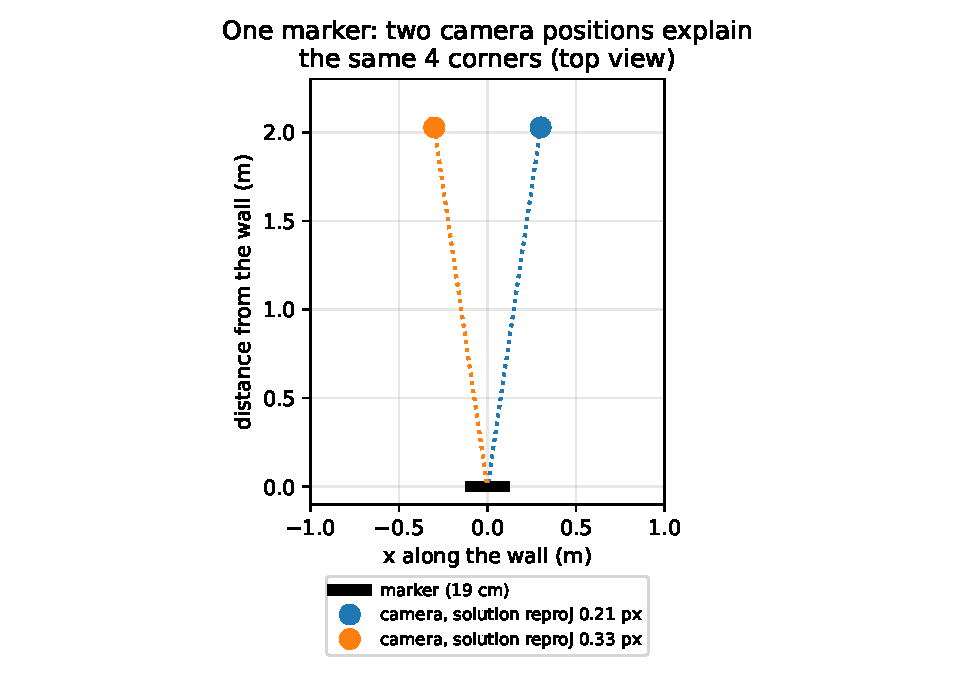
\includegraphics[width=0.55\textwidth]{figures/pnp_mirror.pdf}
\caption{Example 3, top view: two camera positions, 0.62~m apart, explain the same four corners to $0.2$--$0.3$~px.}
\end{figure}

\subsection{Why a solver, and not a formula}

Write eq.~\ref{eq:pinhole} for one corner with the unknowns visible ($r_1^\top, r_2^\top, r_3^\top$ are the rows of
$R$):
\begin{equation}
u_k = f_x \frac{r_1^\top P_k + t_x}{r_3^\top P_k + t_z} + c_x, \qquad
v_k = f_y \frac{r_2^\top P_k + t_y}{r_3^\top P_k + t_z} + c_y .
\end{equation}
Three things make it non-linear, even without any noise:
\begin{enumerate}[leftmargin=*]
\item the unknowns are in a \textbf{fraction} (the division by the depth);
\item $R$ must be a \textbf{rotation}: $R^\top R = I$, $\det R = 1$, i.e.\ 6 quadratic constraints on its 9 entries;
\item the lens \textbf{distortion} $D$ adds polynomial terms ($k_1 r^2 + k_2 r^4 + \dots$) before the pixel.
\end{enumerate}
On top of this, the measurements are noisy: no pose satisfies all the equations exactly, so we look for the pose
that makes the total pixel error as small as possible (least squares):
\begin{equation}
\min_{R,\,t} \; \sum_k \big\lVert \pi(K, D, R P_k + t) - p_k \big\rVert^2 .
\label{eq:pnp-ls}
\end{equation}

\paragraph{The linear shortcut (DLT) and why it is not enough.} Multiplying out the fraction gives equations that are
\emph{linear} in the 12 entries of $M = K[R \mid t]$:
\begin{equation}
(u_k - c_x)\,(r_3^\top P_k + t_z) - f_x\,(r_1^\top P_k + t_x) = 0 .
\end{equation}
Stacking them and taking the SVD solves for $M$ in one shot. But the solution ignores the rotation constraint (the
$R$ found is not a rotation and must be ``straightened'', which adds error), it minimises this algebraic residual and
not the pixel error, it ignores the distortion, and it degenerates when all points are on one plane (one marker). For
a planar marker the linear tool is the \emph{homography} $H \simeq K[r_1\ r_2\ t]$ between the square and the image, which
4 corners determine exactly; IPPE starts from it.

\paragraph{What the code does.}
\begin{center}
\begin{tabular}{@{}p{3.2cm}p{5.6cm}p{5.2cm}@{}}
\toprule
Solver & What it does & When \\
\midrule
\code{IPPE\_SQUARE} & from the homography of one square, returns \emph{both} candidate poses analytically & one marker in view \\
\code{SQPNP} & global minimum of eq.~\ref{eq:pnp-ls} (without distortion) over true rotations, no initial guess & two markers or more \\
\code{solvePnPRefineLM} & Levenberg--Marquardt on eq.~\ref{eq:pnp-ls} with distortion, from the previous solution & always, after the two others \\
\bottomrule
\end{tabular}
\end{center}
One Levenberg--Marquardt step linearises the residuals $r(x)$ (stacked pixel errors, $x$ = the 6 pose parameters,
$J$ = their Jacobian) and moves by
\begin{equation}
\delta x = -\left(J^\top J + \mu I\right)^{-1} J^\top r ,
\end{equation}
a Gauss--Newton step when $\mu$ is small, a small gradient step when $\mu$ is large; a few iterations are enough from the
IPPE/SQPnP start. The error left at the end, the RMS reprojection error, is the quality check: a pose is rejected above
$3$~px with one marker and above $8$~px with several (a marker moved since the mapping, or a wrong id).

\begin{intuition}
The whole chain in one sentence: the detector gives the pixels of corners whose room position is known; the solver
finds the single camera pose that projects those corners onto those pixels with the smallest error; the camera
mount turns the camera pose into the drone pose; that pose, with an uncertainty that grows with the distance and the
pixel error, goes to the EKF on \topic{/aruco/pose}.
\end{intuition}


\section{\texttt{marker\_map.py}: the map, without ROS}

This module has no ROS dependency, so it is shared by the localizer, the map publisher, the fake world and the tools.

\func{Marker}{(id: int, size: float, t: ndarray(3), R: ndarray(3,3))}
A \code{@dataclass}: marker id, side $\ell$ (m), centre $\mathbf t_k$ in \topic{map} and rotation $\mathbf R_k$ whose
columns are the marker's $x,y,z$ axes expressed in \topic{map} (so $\mathbf R_k = {}^m\mathbf R_k$, marker
$\to$ map).

\func{Marker.corners\_map}{(self) -> ndarray(4,3)}
Equation~\eqref{eq:corners}: builds the local corners $(\mp h,\pm h,0)$ with $h=\ell/2$ in the order top-left,
top-right, bottom-right, bottom-left (the order \code{detectMarkers} returns), and returns
\code{(self.R @ local.T).T + self.t}, one row per corner. These are the PnP object points.

\func{rotation\_from\_yaw}{(yaw\_rad) -> ndarray(3,3)}
Fallback orientation for a map without quaternions: an upright marker facing $(\cos\psi,\sin\psi,0)$. It sets
$\mathbf z=(\cos\psi,\sin\psi,0)$ (normal), $\mathbf y=(0,0,1)$ (up), $\mathbf x=\mathbf y\times\mathbf z$ (right, seen
from the front) and stacks them as columns. Example: marker 49, $\psi=90^\circ$: $\mathbf z=(0,1,0)$,
$\mathbf x=(-1,0,0)$, the marker faces $+y$ into the room. Not used with the current map (every entry has \code{q}).

\func{load\_marker\_map}{(path) -> (cfg: dict, markers: dict[int, Marker])}
Reads the YAML with \code{yaml.safe\_load}; default size \code{marker\_size} (0.15 if absent); for every entry builds
a \code{Marker} with \code{R = matrix\_from\_quat(*q)} if \code{q} is present, else \code{rotation\_from\_yaw}. Raises
\code{ValueError} on a duplicate id. Returns the raw dict too (the localizer reads \code{cfg["dictionary"]} from it).

\func{rpy\_from\_matrix}{(R) -> (roll, pitch, yaw)}
ZYX Euler angles such that $\mathbf R = R_z(\psi)R_y(\theta)R_x(\phi)$:
$\theta=-\arcsin R_{31}$ (clamped), $\phi=\operatorname{atan2}(R_{32},R_{33})$, $\psi=\operatorname{atan2}(R_{21},R_{11})$.
Not called anywhere in the repository.

\func{quat\_from\_matrix}{(R) -> (x, y, z, w)}
Standard numerically stable conversion (Shepperd's method): if the trace is positive,
$s=2\sqrt{1+\operatorname{tr}\mathbf R}$, $w=s/4$, $x=(R_{32}-R_{23})/s$, etc.; otherwise it uses the largest diagonal
element to avoid dividing by a small number. Returns ROS order $(x,y,z,w)$.

\func{matrix\_from\_quat}{(x, y, z, w) -> ndarray(3,3)}
The usual unit-quaternion rotation matrix, e.g. $R_{11}=1-2(y^2+z^2)$, $R_{12}=2(xy-zw)$. It does not normalise the
quaternion (see the review).

\func{aruco\_dictionary}{(name) -> cv2.aruco.Dictionary}
\code{cv2.aruco.getPredefinedDictionary(getattr(cv2.aruco, name))}: turns the string \code{"DICT\_6X6\_50"} into the
OpenCV constant. \code{cv2} is imported inside the function so the module can be imported without OpenCV.

\func{marker\_image}{(dictionary\_name, marker\_id, px\_per\_module=100) -> (img, bits)}
Renders a marker image with a one-module white quiet zone, for the fake camera (\file{sim/fake\_world.py}:45) and the
print sheets. \code{bits} is the dictionary's \code{markerSize} (6), the image side is $(6+2)\times 100$~px plus a
100~px white border; it uses \code{generateImageMarker} (OpenCV $\geq$ 4.7) or \code{drawMarker} (4.6).

\section{\texttt{aruco\_localizer.py}: from an image to a pose}

\subsection{Detection}

\func{Detector.\_\_init\_\_}{(self, dict\_name)}
Wraps the two OpenCV ArUco APIs. With OpenCV $\geq$ 4.7 (\code{cv2.aruco.ArucoDetector} exists) it creates
\code{DetectorParameters()}, sets \code{cornerRefinementMethod = CORNER\_REFINE\_SUBPIX} and builds an
\code{ArucoDetector}; with 4.6 it keeps \code{DetectorParameters\_create()} with the same refinement and calls the free
function later. All other detector parameters are OpenCV defaults.

\func{Detector.detect}{(self, gray) -> (corners, ids)}
Calls \code{detectMarkers} on the grayscale image. \code{corners} is a tuple of arrays of shape $(1,4,2)$ (pixels,
float), \code{ids} an $(n,1)$ int array or \code{None}. The rejected candidates (third output) are discarded.

\begin{keypoint}
\textbf{Why grayscale?} The ArUco detector only looks at intensity: a black-and-white pattern has no colour
information, and every step (adaptive threshold, contour finding, bit sampling, sub-pixel refinement) is defined on
a single channel. OpenCV's \code{detectMarkers} expects a gray image (it converts internally if given colour), so
converting once ourselves (\code{cv2.cvtColor(img, cv2.COLOR\_BGR2GRAY)}, $Y = 0.299R+0.587G+0.114B$) makes the cost
explicit and reduces the data handled by 3. The colour image is still kept for the debug overlay.

\textbf{What the detector does} (OpenCV implementation): (1) adaptive thresholding at several window sizes, so it
copes with uneven light; (2) contour extraction and polygon approximation, keeping convex quadrilaterals of
reasonable size; (3) perspective warp of each candidate to a canonical square; (4) Otsu threshold and sampling of the
$8\times8$ cells ($6\times6$ bits plus border), the border must be black; (5) comparison with the 50 codewords in the 4
rotations, accepted if the Hamming distance is within the dictionary's correction capability; this gives the id and
the corner order.

\textbf{What \code{CORNER\_REFINE\_SUBPIX} does.} Step (2) gives corners at integer pixel precision, on a polygon fitted
to a jagged contour. \code{cornerSubPix} then moves each corner inside a small window to the point $\mathbf q$ where
the image gradient is everywhere orthogonal to the vector from $\mathbf q$: for every pixel $\mathbf p_i$ near a true
corner, either $\nabla I(\mathbf p_i)=0$ (flat region) or $\mathbf p_i-\mathbf q$ lies along an edge, so
$\nabla I(\mathbf p_i)^\top(\mathbf p_i-\mathbf q)=0$. Summing the squares gives a $2\times2$ linear system,
$\big(\sum \nabla I\nabla I^\top\big)\mathbf q = \sum \nabla I\nabla I^\top\mathbf p_i$, iterated until it converges.
Precision goes from about 0.5--1~px to about 0.1~px. Since the pose is a least-squares fit to the corners, this
directly improves the pose (and the reprojection test below assumes sub-pixel corners).
\end{keypoint}

\subsection{The node}

\func{ArucoLocalizer.\_\_init\_\_}{(self)}
Declares the parameters and their defaults:
\begin{center}\footnotesize
\begin{tabular}{@{}lll@{}}
\toprule
Parameter & Default & Meaning \\
\midrule
\code{markers\_file} & \code{""} & YAML map, loaded at once by \code{load\_marker\_map} \\
\code{max\_reprojection\_px} & 3.0 & RMS limit for a single-marker pose \\
\code{max\_reprojection\_px\_multi} & 8.0 & RMS limit with 2+ markers, and the ``moved marker'' test \\
\code{debug\_every\_n} & 5 (launch: 3) & one debug image every $n$ frames; 0 = never \\
\code{debug\_scale} & 1.0 (launch: 0.5) & resize factor of the debug image \\
\code{debug\_dir} & \code{""} & if set, save the first 40 debug JPEGs \\
\code{child\_frame} & \code{base\_link\_aruco} & TF child of the raw pose \\
\code{path\_length} & 2000 & maximum poses kept in \topic{/aruco/path} \\
\bottomrule
\end{tabular}
\end{center}
The two thresholds are commented in the code: with several markers, a 1~cm map error is already $\approx 6$~px at
1.6~m ($910\times0.01/1.6=5.7$), while a wrong multi-marker pose is tens of px off; with one marker a mirror pose can
reproject within a few pixels, hence the stricter 3~px. It then builds the \code{Detector} with
\code{cfg.get("dictionary", "DICT\_6X6\_50")}, a \code{CvBridge}, sets \code{K = D = T\_base\_cam = None}, the counters
\code{n} (processed images), \code{ambiguous}, \code{saved} and the dict \code{moved} (marker id $\to$ number of times it
was found inconsistent). It creates a TF \code{Buffer} + \code{TransformListener} (to read the camera mount), a
\code{TransformBroadcaster}, the publishers listed earlier (with depths 10, 2, 5, 5, 2, 5), an empty \code{Path} in
frame \topic{map}, and the two subscriptions: \topic{/tello/camera\_info} (depth 5, \code{on\_info}) and
\topic{/tello/image\_raw} with \textbf{depth 1} (\code{on\_image}) so that only the most recent frame waits.

\func{on\_info}{(self, m: CameraInfo) -> None}
Copies \code{m.k} (row-major $3\times3$) into \code{self.K} and \code{m.d} into \code{self.D} (zeros(5) if the list is
empty). Called for every frame (the driver republishes the info with each image); it simply overwrites the arrays.

\func{camera\_mount}{(self) -> ndarray(4,4) | None}
Returns ${}^b\mathbf T_c$ of equation~\eqref{eq:mount}. The first time, it looks up the TF
\topic{base\_link}$\leftarrow$\topic{tello\_camera\_optical} at \code{Time()} (= latest), converts the quaternion with
\code{matrix\_from\_quat} and the translation into a $4\times4$ matrix, and caches it in \code{self.T\_base\_cam}
(the mount is static: no TF lookup per frame). If the TF is not there yet it returns \code{None} and the frame is
skipped.

\begin{keypoint}
\textbf{What the \topic{tello\_camera\_optical} TF is for.} PnP measures the \emph{camera}; the EKF, the safety layer
and the missions need the \emph{body}. The mount transform says how the two are related: 5~cm ahead of the body
centre (\code{camera\_offset}, default \code{[0.05, 0.0, 0.0]}) and rotated so that the optical axis $z_c$ is the body's
forward axis $x_b$. Without the rotation, the ``camera looking along $z$'' convention of OpenCV would be read as
``drone pointing up''. Having it in TF (rather than hard-coded in the localizer) also lets RViz draw the camera
frustum attached to the drone, and the driver stamps its images with \code{frame\_id = "tello\_camera\_optical"}
(\file{core/driver.py}:69).
\end{keypoint}

\subsection{\texttt{on\_image}: the main callback, step by step}

\func{on\_image}{(self, msg: Image) -> None}
Everything happens in this callback, once per received frame (at most 30~Hz).

\paragraph{1. Preconditions and conversion (lines 119--124).} Returns immediately if no \code{camera\_info} was received
yet or the mount TF is missing. Increments \code{self.n}. \code{imgmsg\_to\_cv2(msg, "bgr8")} converts the driver's
\code{rgb8} message into an OpenCV BGR array (channel swap), then \code{cvtColor(..., COLOR\_BGR2GRAY)} and
\code{detector.detect(gray)}.

\paragraph{2. \topic{/aruco/ids}: what the camera sees (lines 125--132).} For \emph{every} detected marker, mapped or
not: \code{c.reshape(4,2)}, the horizontal position $u = (\bar u_{\text{corners}} - c_x)/c_x$ (about $-1$ at the left
edge, $0$ on the optical axis, $+1.06$ at the right edge since $c_x=466.6<480$), and the longest edge
$s_{\max}=\max_j\lVert \mathbf p_j-\mathbf p_{j-1}\rVert$ (\code{np.roll} pairs each corner with the previous one, so
the four sides are measured). It publishes the string \code{"id:u:size,..."}, e.g. \code{"49:-0.120:96,21:0.410:88"},
or an empty string. This is published on every processed frame, so an empty string means ``nothing seen now''.
\file{missions/patrol.py} uses it to turn towards a marker using the camera only, independently of the map and the pose.

\paragraph{3. Correspondences (lines 134--142).} For each detected id present in the map and not blacklisted
(\code{self.moved.get(id,0) >= 3}), it appends the four map corners \code{mk.corners\_map()} to \code{obj}, the four
image corners to \code{imgp} and the id to \code{used}. Detected ids absent from the map (e.g. 13--16, 48) are
ignored here. The corner order is consistent on both sides: the detector returns them top-left first in the marker's
own orientation, and \code{corners\_map} uses the same order.

\paragraph{4. Moved marker (lines 143--144).} With at least 3 markers, \code{drop\_moved\_marker} may remove one
marker inconsistent with the others (section~\ref{sec:moved}).

\paragraph{5. Nearest marker (lines 146--150).}\label{sec:nearest} If at least one marker is used:
\begin{equation}
d_{\text{near}} = \min_{k\in\text{used}} \frac{f_x\,\ell_k}{\max(s_{\max,k},\,1)} .
\end{equation}
The longest side is used because foreshortening (seeing the marker at an angle) only shortens the sides; the longest
one is the closest to the frontal size. This is a monocular range-from-size estimate, independent of the pose (it
does not care if PnP fails later), but it does depend on the map for $\ell_k$ and only uses mapped, non-blacklisted
markers. It is published on \topic{/aruco/nearest\_marker}. The driver's \code{wall\_guard} (\file{core/safety.py}:351--365)
forbids forward motion and backs off ($fb\leq -12$) below \code{min\_wall = 0.7}~m (a marker 246~px wide) and scales
the forward command down linearly between 0.70 and 0.85~m; it ignores readings older than 0.4~s, which is how ``no
marker'' is handled, since nothing is published in that case.

\paragraph{6. Pose (lines 151--163).} The object and image points are concatenated into $N\times3$ and $N\times2$
\code{float64} arrays, $N=4n$. With \textbf{one} marker, \code{single\_marker\_pose} (IPPE + disambiguation); on failure
\code{ambiguous} is incremented and the frame gives no pose. With \textbf{two or more}, one joint call
\code{cv2.solvePnP(obj\_pts, img\_pts, K, D, flags=SOLVEPNP\_SQPNP)}. If a solution exists it is refined by
\code{solvePnPRefineLM} over the same points.

\begin{keypoint}
\textbf{Several markers: one problem, not an average.} All visible markers contribute their corners, expressed in the
common \topic{map} frame, to the same sum~\eqref{eq:pnp}: with 5 markers, 20 correspondences and one rotation and
translation to find. Three reasons this beats estimating 5 poses and averaging them: (i) the corners are spread over
a large part of the image and of the wall, so the effective ``baseline'' is the distance between markers (metres)
rather than one marker side (19~cm); this conditions orientation and depth far better; (ii) markers on different
walls (non-coplanar points) remove the planar ambiguity entirely; (iii) averaging rotations is not even well defined
without care, whereas the joint solution is one rotation ${}^c\mathbf R_m$ from which the body orientation follows by
equation~\eqref{eq:body}. Orientation is not computed separately: the yaw comes from the same least-squares fit as the
position.
\end{keypoint}

\paragraph{7. Reprojection error and transforms (lines 164--171).} \code{projectPoints} re-projects the object points
with the refined pose and the RMS pixel error is
\begin{equation}
e_{\text{RMS}} = \sqrt{\frac{1}{N}\sum_{i=1}^{N}\big\lVert \mathbf p_i - \pi(\mathbf X_i;{}^c\mathbf R_m,{}^c\mathbf t_m,
\mathbf K,\mathbf D)\big\rVert^2}\quad[\text{px}] .
\label{eq:rms}
\end{equation}
It is the square root of the PnP cost divided by $N$: the typical distance between where a corner \emph{is} and where
the map and the pose say it \emph{should be}. When the map, the calibration and the detection all agree, it is a
fraction of a pixel to about 2~px; a wrong pose, a misidentified marker or a moved marker gives tens or hundreds of px.
Then \code{Rodrigues} gives ${}^c\mathbf R_m$, the code builds ${}^m\mathbf T_c$ (rotation $\mathbf R^\top$, translation
$-\mathbf R^\top\mathbf t$), ${}^m\mathbf T_b = {}^m\mathbf T_c\,({}^b\mathbf T_c)^{-1}$ (equation~\eqref{eq:body}) and the
mean camera-to-corner distance
$\bar d = \frac1N\sum_i \lVert \mathbf X_i - \mathbf c\rVert$ used by the covariance.

\begin{lstlisting}
R_cm, _ = cv2.Rodrigues(rvec)  # map -> camera
T_map_cam = np.eye(4)
T_map_cam[:3, :3] = R_cm.T
T_map_cam[:3, 3] = (-R_cm.T @ tvec).ravel()
T_map_base = T_map_cam @ np.linalg.inv(self.T_base_cam)
dist = float(np.mean(np.linalg.norm(obj_pts - T_map_cam[:3, 3], axis=1)))
\end{lstlisting}

\paragraph{8. Acceptance (lines 172--173).} The limit is 3~px for one marker, 8~px for several; the pose is accepted
iff $e_{\text{RMS}}\leq$ limit \textbf{and} \code{plausible(position, n)} (section~\ref{sec:plausible}). Because of
Python's short-circuit \code{and}, \code{plausible} is only called (and only updates its memory) when the error test
passed.

\paragraph{9. Publishing (lines 174--179).} If accepted: store \code{\_last\_cam = (now, camera position)} (used by the
single-marker disambiguation), \code{publish(...)} and \code{publish\_viz(...)}, all with the \emph{image} stamp
\code{msg.header.stamp}. Then, whether accepted or not, every \code{debug\_every}-th processed frame goes to
\code{publish\_debug}.

\subsection{Rejections and safeguards}

\func{reprojection}{(self, obj: list, imgp: list) -> float}
Helper for the moved-marker test: concatenates the given markers' points, runs the same SQPnP + LM pipeline as the
main path and returns $e_{\text{RMS}}$ (equation~\eqref{eq:rms}), or $+\infty$ if \code{solvePnP} fails.

\func{drop\_moved\_marker}{(self, obj, imgp, used) -> (obj, imgp, used)}\label{sec:moved}
Handles a marker that is no longer where the map says. Such a marker poisons the joint PnP: on Nov~13 marker 39 had
fallen and been put back elsewhere; facing that wall, 6 markers gave 438~px, every pose was rejected, the drone flew
4.5~s blind, then 39 alone gave a pose 0.8~m too high and the mission landed. The algorithm, for $n\geq3$ markers:
\begin{enumerate}
\item $e_{\text{all}}=$ \code{reprojection}(all). If $e_{\text{all}}\leq 8$~px, keep everything.
\item Otherwise compute the leave-one-out errors $e_{-k}$ for $k=1..n$ (PnP without marker $k$), and
  $k^\ast=\arg\min_k e_{-k}$.
\item If $e_{-k^\ast} > 8$~px, removing one marker does not fix it (bad frame, several errors): return everything and let
  the normal rejection discard the frame.
\item Otherwise marker $k^\ast$ is the culprit: increment \code{moved[k*]}; at exactly 3 it logs a warning
  (``does not match the map (moved since the capture?): ignored from now on. Re-map it''), and from then on line 138
  skips it for the rest of the run. Return the lists without $k^\ast$.
\end{enumerate}
Why at least 3 markers: with 2, removing either one leaves a single marker that always fits itself, so the test
cannot tell which one is wrong; with 3 or more the remaining ones must agree with each other. The cost is $n+1$ PnP
solves when the markers disagree and 1 extra solve when they agree (step 1 is repeated by the main path afterwards).

\func{single\_marker\_pose}{(self, corners, mk, min\_ratio=3.0, max\_tilt\_deg=30.0) -> (ok, rvec, tvec)}\label{sec:single}
\textbf{The ambiguity.} Four coplanar points of a small square seen from a distance project almost affinely. Under an
affine camera, a plane tilted by $+\theta$ and by $-\theta$ about an axis in the image plane produces the same image,
so there are two poses (a ``flip'') with almost the same reprojection error; perspective breaks the tie only weakly
when the marker is small in the image (a few tens of pixels). The two poses put the camera at two different places,
mirrored about the marker's line of sight, often tens of centimetres to more than a metre apart (1.4~m errors were seen
with the fake drone when SQPnP converged to the mirror pose, comment on line 155).

\textbf{Solver.} IPPE on the marker's \emph{local} corners $(\mp h,\pm h,0)$, through
\code{solvePnPGeneric(..., flags=SOLVEPNP\_IPPE\_SQUARE)}, which returns $n\leq2$ solutions
$({}^c\mathbf R_k,{}^c\mathbf t_k)$ and their reprojection errors $e$ (an OpenCV exception or zero solutions returns
\code{ok=False}). Each solution is converted from ``marker $\to$ camera'' to ``map $\to$ camera'' using the map pose
of the marker: since $\mathbf X_k = \mathbf R_k^\top(\mathbf X_m-\mathbf t_k)$,
\begin{equation}
\mathbf X_c = {}^c\mathbf R_k\mathbf R_k^\top \mathbf X_m + \big({}^c\mathbf t_k - {}^c\mathbf R_k\mathbf R_k^\top\mathbf t_k\big)
\ \Rightarrow\
{}^c\mathbf R_m = {}^c\mathbf R_k\mathbf R_k^\top,\quad {}^c\mathbf t_m = {}^c\mathbf t_k - {}^c\mathbf R_m\mathbf t_k,
\end{equation}
camera position $\mathbf c = -{}^c\mathbf R_m^\top\,{}^c\mathbf t_m$, and camera ``down'' axis in the map
$\mathbf y_c = $ second column of ${}^c\mathbf R_m^\top$. The camera tilt is the angle between that axis and gravity,
$\text{tilt} = \arccos(-y_{c,z})$ (argument clamped to $[-1,1]$): 0 for a level camera.

\textbf{Choice}, in order:
\begin{enumerate}
\item drop candidates with tilt $>30^\circ$ (the Tello camera is level and the drone tilts less than $15^\circ$); none
  left $\Rightarrow$ reject;
\item sort by error; if only one remains, take it;
\item if $e_2/\max(e_1,10^{-6})\geq 3$, the best one is clearly better: take it;
\item if the two camera positions are less than 0.15~m apart, take the best (head-on view, where both solutions are
  nearly the same pose; rejecting these lost the drone in front of marker 10 on Nov~10);
\item otherwise use history: if the last accepted camera position \code{\_last\_cam} is less than 1.0~s old, take the
  candidate closest to it, provided it is within 0.4~m; else reject.
\end{enumerate}
The chosen ${}^c\mathbf R_m$ goes back to an \code{rvec} with \code{Rodrigues}; the caller then refines it with LM over
the \emph{map} corners (identical to the local ones up to a rigid change of frame) and applies the 3~px test.

\func{plausible}{(self, pos, n\_markers, max\_jump=0.5, window=0.5) -> bool}\label{sec:plausible}
A jump gate for single-marker poses, catching a flip the rules above missed. With \code{\_last\_ok = (t, position)}
the last accepted body position: if $n=1$ \textbf{and} the last one is less than 0.5~s old \textbf{and}
$\lVert \mathbf p - \mathbf p_{\text{last}}\rVert > 0.5$~m, reject (and increment \code{ambiguous}). Otherwise accept and
store the new pose. Poses from 2+ markers are always accepted and therefore \emph{re-anchor} the gate. Note the time
used is the node clock at processing time, not the image stamp. At 1~m/s the drone moves 0.5~m in 0.5~s, so the gate
cannot reject a genuine motion between two consecutive frames (33~ms).

\subsection{Publishing}

\func{publish}{(self, stamp, T, err, dist, n\_markers) -> None}
Builds the \code{PoseWithCovarianceStamped} in frame \topic{map}, stamp = image stamp, position = ${}^m\mathbf t_b$,
orientation = \code{quat\_from\_matrix}$({}^m\mathbf R_b)$. The covariance is a heuristic: a pixel error $e$ at
distance $\bar d$ is a metric error $e\bar d/f_x$; it is inflated by 1.5, the error is floored at 0.3~px, and divided by
$\sqrt n$ as if markers were independent measurements:
\begin{equation}
\sigma_p = \max\!\Big(0.01,\ \frac{1.5\,\max(e,0.3)\,\bar d}{f_x\sqrt n}\Big)\ \text{m},\qquad
\sigma_\psi = \max\!\Big(0.5^\circ,\ \frac{\sigma_p}{\max(\bar d,0.3)}\Big).
\end{equation}
The $6\times6$ row-major covariance is diagonal: indices 0, 7, 14 ($x,y,z$) get $\sigma_p^2$, indices 21, 28, 35
(roll, pitch, yaw) get $\sigma_\psi^2$. Examples with $f_x=910.5$: $e=0.5$, $\bar d=2$, $n=4$ gives 0.8~mm, so the 1~cm
floor applies (the usual case); $e=6$~px, $\bar d=3$~m, $n=3$ gives $\sigma_p=1.7$~cm and $\sigma_\psi=0.33^\circ$, so
the $0.5^\circ$ floor ($8.7$~mrad) applies. The EKF reads only \code{covariance[0]} and \code{covariance[35]}
(\file{core/ekf\_node.py}:71--72) as the position and yaw standard deviations of its update. The message is stored in
\code{self.last\_pose}. A \code{TransformStamped} with the same header, child \code{self.child\_frame}
(\topic{base\_link\_aruco}) and the same pose is broadcast on \topic{/tf}: the EKF owns \topic{base\_link}, so the raw
measurement gets its own frame for comparison in RViz.

\func{publish\_viz}{(self, stamp, cam\_pos, used) -> None}
RViz helpers. (i) Appends a \code{PoseStamped} of \code{last\_pose} to \code{self.path}, keeps the last
\code{path\_max} (2000) poses (\code{del poses[:-2000]}), and publishes the whole path at most every 0.2~s (5~Hz).
(ii) A \code{LINE\_LIST} marker (namespace \code{sight}, id 0, width 1~cm, green $(0.1,1,0.2)$, alpha 0.9) with one
segment from the camera position to the centre of each used marker; lifetime 0.5~s, so the lines vanish half a second
after the markers are lost (the marker is only re-published on accepted frames).

\func{publish\_debug}{(self, msg, img, corners, ids, ok, err, used) -> None}
Copies the colour image, draws all detections (\code{drawDetectedMarkers}: outlines and ids, mapped or not), writes
``\code{<n> markers reproj <e>px OK}'' in green or ``\code{REJECTED}'' in red ($(0,0,255)$ in BGR), or ``no marker''
if none was used; resizes by \code{debug\_scale} with \code{INTER\_AREA} (the right filter for shrinking); converts
back to a \code{bgr8} message with the original header and publishes it. If \code{debug\_dir} is set, the first 40
images are also written as \file{debug\_<n>.jpg}. With the launch values (every 3rd frame, scale 0.5) the topic runs at
about 10~Hz with $480\times360$ images, i.e.\ 0.5~MB per message instead of 2~MB, 12 times less bandwidth than
full-rate full-size.

\func{main}{() -> None}
\code{rclpy.init}, create the node, \code{spin} until Ctrl+C or external shutdown, destroy, \code{shutdown} if still
running. Single-threaded executor: \code{on\_info} and \code{on\_image} never run concurrently.

\section{\texttt{marker\_map\_publisher.py}: static frames and RViz scene}

This node computes nothing at run time. It publishes once what never changes (static TFs, latched markers) and
republishes a few RViz markers periodically so that a late or restarted RViz always shows them.

\func{camera\_mount\_rotation}{() -> ndarray(3,3)}
Returns ${}^b\mathbf R_c$ of equation~\eqref{eq:mount}, built as \code{np.column\_stack([[0,-1,0],[0,0,-1],[1,0,0]])}:
the optical $x,y,z$ axes written in body coordinates.

\func{make\_tf}{(stamp, parent, child, t, R) -> TransformStamped}
Fills a \code{TransformStamped} with translation \code{t} and the quaternion of \code{R}.

\func{MarkerMapPublisher.\_\_init\_\_}{(self)}
Parameters: \code{markers\_file}, \code{camera\_offset} (default \code{[0.05, 0.0, 0.0]}), \code{flight\_zone\_file},
\code{room\_mesh}. In order:
\begin{enumerate}
\item Loads the map and builds one static TF \topic{map}$\to$\topic{aruco\_<id>} per marker (${}^m\mathbf T_k$, i.e.
  translation $\mathbf t_k$, rotation $\mathbf R_k$) plus \topic{base\_link}$\to$\topic{tello\_camera\_optical}; sends the
  45 transforms in one \code{StaticTransformBroadcaster.sendTransform} call (static TFs go on the latched
  \topic{/tf\_static} topic, so they are received by any later listener, including the localizer's
  \code{camera\_mount}).
\item Publishes \code{map\_markers} on \topic{/aruco/map\_markers} with a latched QoS (depth 1, transient local).
\item Publishes \code{body\_markers} on \topic{/tello/body\_markers} (latched), stamped with time 0, and re-publishes
  it every 1.0~s with a timer.
\item If \code{flight\_zone\_file} is set: loads it; creates \topic{/room/flight\_zone}. If the file has a \code{boxes}
  key (3D zone mode), only the green boxes of that file are drawn; otherwise a yellow box $(1,0.8,0)$ from its
  \code{x/y/z\_min/max} (the zone the driver enforces; band file: $x\in[-0.86,0.94]$, $y\in[0.36,2.76]$,
  $z\in[1.70,2.00]$) plus, if the sibling \file{flight\_zone\_3d.yaml} exists, its boxes in green $(0.1,0.85,0.25)$
  (the proposed L-shaped 3D zone). Published once and every 2.0~s. If the file names a \code{grid\_file}, calls
  \code{publish\_free\_space} with \code{margin} (0.25 in the band file; default 0.35). Any error only logs a warning.
\item If \code{room\_mesh} is set: one \code{MESH\_RESOURCE} marker on \topic{/room/mesh} in frame \topic{map}, scale 1,
  \code{mesh\_resource = "file://<path>"}, colour $(0,0,0,0)$ with \code{mesh\_use\_embedded\_materials = True}: an
  all-zero colour tells RViz to use the scan's own texture without tinting. Latched, published once.
\end{enumerate}

\func{publish\_free\_space}{(self, npz, margin, qos) -> None}
Creates the latched \topic{/room/free\_space} publisher and publishes \code{free\_space\_grid(npz, margin)} once.

\func{free\_space\_grid}{(npz, margin) -> OccupancyGrid}
Loads the \code{.npz} produced by \file{tools/free\_zone.py} from the room scan: \code{clearance} (a 2D array, for
each $5$~cm cell the horizontal distance in metres to the nearest scanned surface in the height band, computed with a
distance transform; cells outside the main free region get a clearance below the margin), \code{cell} (0.05~m),
\code{x0}, \code{y0} (grid origin, here $(-1.560,-1.239)$). For the band grid, \code{clearance} is
$99\times75$ (rows $=y$, columns $=x$), i.e.\ $3.75\times4.95$~m. The message has
\code{resolution = cell}, \code{width} = columns, \code{height} = rows, origin at $(x_0,y_0)$ with identity
orientation, and data \code{100} where $\text{clearance}<\text{margin}$ (no-fly) and \code{0} elsewhere, flattened
row-major (x fastest), which is the \code{OccupancyGrid} convention. About 75\,\% of the cells are no-fly (most of the
rectangle is outside the room or near furniture).

\textbf{How it looks in RViz.} \file{real.rviz} shows it with a \code{Map} display, colour scheme \code{map}, alpha
0.35, at $z=0$ (the floor). In that scheme 100 is black and 0 is light grey: the black cells are where the driver's
free-space guard will not let the drone go (closer than the margin to an obstacle), the light ones where it may fly.
Because the layer is 35\,\% opaque, the free cells take the colour of what lies under or behind them (the textured
mesh, the translucent green 3D zone seen from above), which is why the ``free'' part can look tinted rather than
white.

\func{map\_markers}{(self, stamp) -> MarkerArray}
For each marker, three visual markers in the marker's own TF frame \topic{aruco\_<id>} (so they are placed by TF, not
by copying coordinates): a white sheet (\code{CUBE} $1.5\ell\times1.5\ell\times4$~mm at $z=-4$~mm, i.e.\ just
behind, on the wall side), a black square (\code{CUBE} $\ell\times\ell\times6$~mm) and the id as yellow
\code{TEXT\_VIEW\_FACING} (height 0.14~m) at $y=1.1\ell$ above the marker, $z=3$~cm in front. Plus a white 8~cm sphere
at the \topic{map} origin. Namespaces \code{aruco\_sheet}, \code{aruco}, \code{aruco\_id}, \code{origin}, id = marker id.

\func{body\_markers}{(self, stamp) -> MarkerArray}
A drone drawn about twice its real size, attached to \topic{base\_link}: a grey body \code{CUBE}
$0.20\times0.18\times0.08$~m; four propellers (\code{CYLINDER} diameter 0.14~m, 1~cm thick) at
$(\pm0.13,\pm0.13,0.045)$, front ones red and rear ones dark grey (so the heading is visible); a red \code{ARROW} 0.35~m
long along $x_b$; and the camera frustum as a cyan \code{LINE\_LIST} in \topic{tello\_camera\_optical}: the 4 edges
from the optical centre to a 1~m-deep rectangle of half-sizes $\tan 27.8^\circ$ and $\tan 21.5^\circ$ (the FOV of the
calibration) and the 4 edges of that rectangle. Stamp 0 means ``use the latest transform'': \topic{base\_link} moves
(published by the EKF), and a fixed old stamp would ask TF for a pose in the past. They are on a separate topic from
\topic{/aruco/map\_markers} so that the marker display does not show a ``no transform'' warning before the first
\topic{base\_link} pose exists.

\func{point}{(x, y, z) -> Point}
Builds a \code{geometry\_msgs/Point} from three floats.

\func{viz}{(stamp, frame, ns, mid, mtype, scale, rgba, x=0, y=0, z=0) -> Marker}
Factory for a \code{visualization\_msgs/Marker} with action \code{ADD}, the given frame, namespace, id, type, scale,
colour and position, identity orientation, and \code{frame\_locked = True}: RViz re-transforms the marker every
frame with the current TF, so markers attached to \topic{base\_link} follow the drone.

\func{box\_markers}{(arr, ns, i, xs, ys, zs, rgb) -> None}
Appends a box in \topic{map}: a translucent \code{CUBE} (alpha 0.3, id $2i$) and a \code{LINE\_LIST} of its 12 edges
(width 2.5~cm, opaque, id $2i+1$). The 8 corners are the products $\{x_0,x_1\}\times\{y_0,y_1\}\times\{z_0,z_1\}$; two
corners form an edge iff they differ in exactly one coordinate ($\binom82=28$ pairs, 12 of them edges). The comment
explains the thick edges: a bare transparent cube vanished inside the textured scan.

\func{main}{() -> None}
Same pattern as the localizer.

\section{Communication and latency}

\begin{itemize}
\item \textbf{Stamps.} The driver stamps each image when it reaches the PC (\file{core/driver.py}:285) with
  \code{frame\_id = tello\_camera\_optical} and gives the same stamp to the \code{camera\_info}. The localizer copies
  that stamp to the pose, the TF, the path and the debug image. The pose therefore describes the drone about 0.2~s in
  the past (video latency); the EKF applies it at that time and re-propagates to now.
\item \textbf{No queueing of old frames.} The image subscription has depth 1 (KEEP\_LAST): if \code{on\_image} is still
  busy when new frames arrive, the older waiting frame is overwritten, never processed late. Lag cannot accumulate; the
  pose rate simply drops below 30~Hz if processing is slow.
\item \textbf{Cheap per-frame work.} The mount TF is read once and cached; the map corners are computed with one
  $3\times3$ product per marker; PnP on 8--24 points costs well under a millisecond. The dominant costs are the
  colour conversions and \code{detectMarkers} on the $960\times720$ image, plus the extra PnP solves of
  \code{drop\_moved\_marker}.
\item \textbf{Throttled visual outputs.} Debug image every \code{debug\_every\_n} = 3 frames, scaled by 0.5, publisher
  depth 2; path at 5~Hz; sight lines expire after 0.5~s. The recorder subscribes the debug image with depth 1 and saves
  at most one per second.
\item \textbf{Latched static data.} Everything constant (\topic{/tf\_static}, map markers, mesh, free space, zones) is
  published with transient-local durability, so it costs nothing per frame and late subscribers still get it.
\end{itemize}

\section{Questions answered}

\begin{description}[style=nextline]
\item[Why convert to gray? What does corner refine / subpix do?] The detector is defined on intensity only; one
  channel is all it needs. Sub-pixel refinement moves each corner to where the image gradients are orthogonal to the
  corner-to-pixel vectors, solving a $2\times2$ least-squares system: about 0.1~px precision instead of $\sim$1~px,
  which the pose inherits (Keypoint in section ``Detection'').
\item[How is the drone located once a marker is detected?] The four detected corners (image points) are matched to the
  four corners of that marker in the map (object points, equation~\eqref{eq:corners}); PnP (equation~\eqref{eq:pnp})
  finds \code{rvec, tvec} $= ({}^c\mathbf R_m,{}^c\mathbf t_m)$; the camera pose is its inverse; the body pose is
  ${}^m\mathbf T_b={}^m\mathbf T_c({}^b\mathbf T_c)^{-1}$. One marker uses IPPE (two solutions, disambiguated); several
  use SQPnP; both are refined with LM.
\item[Does it use how many pixels the marker takes?] Only for \topic{/aruco/nearest\_marker} ($d=f_x\ell/s_{\max}$) and
  \topic{/aruco/ids}. In PnP the apparent size is implicit: the metric object points and the focal length in pixels
  force the depth. That is how the calibration gives distance: $f_x=910.5$~px converts between pixel sizes and angles,
  and $\ell=0.1889$~m fixes the scale.
\item[Several markers?] One joint PnP over all corners in the \topic{map} frame; one rotation and one translation, from
  which position and orientation both follow; much better conditioned than one marker and free of the flip ambiguity.
\item[Reprojection RMS?] Equation~\eqref{eq:rms}: RMS pixel distance between detected corners and corners projected with
  the solved pose. Thresholds 3~px (one marker), 8~px (several).
\item[Moved marker?] Leave-one-out test with 3+ markers: if all together exceed 8~px but removing one brings it under
  8~px, that marker is dropped for this frame; after 3 such frames it is ignored for the rest of the run, with a
  warning.
\item[Single-marker ambiguity?] IPPE's two mirror poses; drop tilts $>30^\circ$, take the better if 3 times better or
  if both are within 15~cm, else the one closer (and within 0.4~m) to the pose of less than 1~s ago, else reject.
\item[Plausible / jump?] A single-marker pose more than 0.5~m from an accepted pose less than 0.5~s old is rejected;
  multi-marker poses always pass and re-anchor.
\item[Where is it published, who listens, how is lag limited?] See the topic table and the previous section: EKF,
  driver wall guard, patrol, recorder, RViz; depth-1 image queue, cached mount, throttled and scaled debug image.
\item[What is the camera mount TF for?] To turn a camera pose into a body pose (equation~\eqref{eq:mount}) and to
  draw the camera in RViz.
\item[What is \code{marker\_map\_publisher} for?] Static TFs of the markers and of the camera mount, and the RViz
  scene: markers (\topic{/aruco/map\_markers}), drone body and frustum (\topic{/tello/body\_markers}), room scan
  (\topic{/room/mesh}), flight zones (\topic{/room/flight\_zone}, yellow enforced, green 3D proposal) and the free-space
  grid (\topic{/room/free\_space}, black = no-fly).
\end{description}

\section{Code review notes}

\begin{review}
All items were checked in the current code; none was changed.
\begin{enumerate}
\item \textbf{Stale comment} -- \file{aruco\_localizer.py}:62--63 says the real-drone launch sets \code{child\_frame}
  to \code{base\_link} ``until the EKF exists''; \file{real.launch.py}:57 sets \code{base\_link\_aruco} and the EKF is
  always launched. Misleading when debugging TF.
\item \textbf{Duplicate PnP solve (latency)} -- \file{aruco\_localizer.py}:143--144 with 197 and 160--163: with 3+
  markers, \code{drop\_moved\_marker} solves SQPnP+LM on all markers, then the main path solves exactly the same problem
  again; when markers disagree, $n+2$ solves per frame. Returning the pose from \code{reprojection} would remove one
  solve every frame.
\item \textbf{Moved-marker counter never decays} -- \file{aruco\_localizer.py}:204--205, 138: three transient
  mismatches (motion blur, a bad corner) at any moment of the run blacklist a correct marker until restart; nothing
  resets \code{self.moved}. A decay or ``consecutive frames'' rule would be safer. Also, with exactly 2 disagreeing
  markers (line 143) there is no recovery: the frame is lost.
\item \textbf{Proximity sensor depends on the map} -- \file{aruco\_localizer.py}:146--150 versus the comment at 79--80
  (``no map, no pose''): $d_{\text{near}}$ is computed only over \code{used}, i.e. mapped and non-blacklisted markers,
  after \code{drop\_moved\_marker}. A blacklisted or unmapped marker on a wall no longer feeds the wall guard; using
  all detections with the default \code{marker\_size} would match the stated intent.
\item \textbf{Silent startup drop} -- \file{aruco\_localizer.py}:119--120: without \code{camera\_info} or the mount TF
  every frame is discarded without any log; a throttled warning would make a missing \code{marker\_map\_publisher}
  obvious.
\item \textbf{Double colour conversion} -- \file{aruco\_localizer.py}:122--123: \code{rgb8} $\to$ \code{bgr8} copy, then
  BGR $\to$ gray. The BGR image is needed only every 3rd frame for the debug overlay; converting \code{rgb8} directly
  with \code{COLOR\_RGB2GRAY} and building BGR only when debugging saves a full-frame copy per frame.
\item \textbf{\code{u} normalisation} -- \file{aruco\_localizer.py}:129 divides by $c_x=466.6$ rather than half the
  width, so the documented ``$-1..+1$'' range is really about $[-1, 1.06]$. Harmless but surprising to \file{missions/patrol.py}.
\item \textbf{Dead code} -- \code{self.ambiguous} (\file{aruco\_localizer.py}:70, 158, 264) is incremented but never read
  or logged; \code{rpy\_from\_matrix} (\file{marker\_map.py}:57--62) is never called; the
  \code{SOLVEPNP\_ITERATIVE} fallback (lines 160, 184) cannot trigger on OpenCV $\geq$ 4.5.3, which both supported
  versions are.
\item \textbf{Duplicated corner layout} -- \file{aruco\_localizer.py}:220--221 re-implements the local corners of
  \file{marker\_map.py}:24--25; a change of corner order in one place would silently break IPPE. Factor into one helper.
\item \textbf{Lazily created attributes} -- \code{\_last\_cam} (line 175), \code{\_last\_ok} (266), \code{last\_pose}
  (287) are created on first use and read with \code{getattr}; initialising them in \code{\_\_init\_\_} is clearer.
  The \code{std\_msgs} imports inside \code{\_\_init\_\_} (lines 81, 86) also belong at the top.
\item \textbf{Debug text with NaN} -- \file{aruco\_localizer.py}:327: when a single marker is ambiguous, \code{err}
  stays \code{nan} and the overlay reads ``reproj nanpx REJECTED''; printing ``ambiguous'' would be clearer in the
  flight frames.
\item \textbf{Covariance model} -- \file{aruco\_localizer.py}:272--284: isotropic $\sigma_p$ although PnP depth error
  is much larger than lateral error ($\delta Z/Z=\delta s/s$ versus $Z/f_x$ per pixel); roll and pitch get the yaw
  value; no correlations. Acceptable because the EKF only reads entries 0 and 35 (\file{core/ekf\_node.py}:71--72), but the
  1~cm floor dominates almost always, so the EKF effectively sees a constant $\sigma_p$.
\item \textbf{Tilt check not re-applied after LM} -- \file{aruco\_localizer.py}:163 refines the IPPE choice with LM
  but the $30^\circ$ tilt rule (238) is not re-checked on the refined pose; only the 3~px and jump tests remain.
\item \textbf{Path bandwidth} -- \file{aruco\_localizer.py}:302--307: the whole path (up to 2000 poses, about
  0.2~MB) is re-sent at 5~Hz, yet \file{real.rviz} displays \topic{/ekf/path}, not \topic{/aruco/path}.
\item \textbf{Quaternions not normalised} -- \file{marker\_map.py}:83--88 with the 4-decimal quaternions of
  \file{markers.yaml} (e.g. id 1: $\lVert q\rVert^2=1.00008$) gives a slightly non-orthonormal $\mathbf R_k$ (scale
  error $\sim10^{-4}$, i.e. $<0.02$~mm on a corner). Negligible, but normalising costs one line.
\item \textbf{Unmeasured marker} -- \file{config/markers.yaml}:58 (id 18) was placed by hand; any error in it raises the
  joint reprojection error and may make \code{drop\_moved\_marker} blacklist it (or, with 2 markers, lose frames).
  Re-measure it with \file{tools/room\_mapper.py}.
\item \textbf{Unclosed files} -- \file{marker\_map\_publisher.py}:67, 79 use \code{yaml.safe\_load(open(...))}
  without closing; use \code{with open(...)}.
\end{enumerate}
\end{review}
